\documentclass{sig-alternate}
\usepackage[utf8]{inputenc}

\usepackage{graphicx} % Allows including images
\usepackage{booktabs} % Allows the use of \toprule, \midrule and \bottomrule in tables
%\usepackage{hyperref} % Allows to put hyperlinks.
\usepackage{color}
\usepackage{listings}
\usepackage[english]{babel}
\usepackage{subcaption}
\usepackage{float}
\usepackage{amsmath}
\usepackage{pgfplots}
\usepackage{authblk}
\usepackage[hidelinks]{hyperref}
\usepackage{multicol} % This is so we can have multiple columns of text side-by-side
% \columnsep=100pt % This is the amount of white space between the columns in the poster
% \columnseprule=3pt % This is the thickness of the black line between the columns in the poster
%opening
\title{Hilbert Curve based Flexible Dynamic Partitioning Scheme for Adaptive Scientific Computations}
\author{Milinda Fernando, Hari Sundar (Advisor)}
\affil{School of Computing, University of Utah}
\date{}

\begin{document}

\maketitle

\begin{abstract}

  Space Filling Curves (SFC) are commonly used by the HPC community for
  partitioning data\cite{campbell2003,devine2005,sundar2007} and for resource
  allocations\cite{bender51,slurm}. Amongst the various SFCs, Hilbert curves
  have been found to be in general superior to the more ubiquitous Morton or
  Z-Curve \cite{campbell2003}. However, their adoption in large-scale HPC
  codes, especially for partitioning applications, has not been as common as
  Morton curves due to the computational complexity associated with the Hilbert
  ordering. In this work, we present an alternative algorithm for computing the
  Hilbert ordering that can be implemented almost as efficiently as the Morton
  ordering. 
  %Additionally, being based on the concept of the {\em nearest common
  %ancestor}---a fundamental property of all SFCs---the algorithm can be applied
  %to all SFCs. 
  We also propose a modification to the standard SFC based
  partitioning algorithm that tolerates small (user-specified) work-load imbalance 
  to obtain larger savings in communication costs. This
  allows us to obtain significant improvements in
  partition quality while using Hilbert ordering.
%We also present comparisons of Morton and Hilbert curve based partitions for
  %adaptive meshes using two partitioning schemes demonstrating the superiority
  %of Hilbert ordering. 
\end{abstract}

\section{Introduction}

Load balancing and partitioning are critical when it comes to parallel
computations. Generally partitioning involves equally dividing the work and
data among the processors, reducing processor idle time and communication
costs. 
% Partitioning can be done statically or dynamically.
%In this research we are focused on developing an efficient flexible dynamic
%partitioning scheme, based on the Hilbert curve, targeted at adaptive-mesh
%computations. 
As we march towards exascale machines, the cost of data movement and
load-imbalances therein are a major bottleneck for achieving scalability. We
propose an alternative SFC-based partitioning scheme where we allow some
(user-specified) flexibility in the work assignment, so as to minizmize the
data-dependencies across partitions. Effectively, we allow the flexibility in
minimizing the communication load-imbalance at the cost of a marginal increase
in work load-imbalance. The traditional SFC-based partitioning can be recovered
by setting the flexibility to zero.  

One of the main advantage of SFC based partitioning is the preservation of
geometric locality of objects between processors. Depending on the SFC (i.e.
Morton, Moore, Hilbert) that used for partitioning, the amount of locality
preserved differs \cite{bader2012}.  
Most SFC based partitioning---especially for adaptive meshing---use the
Morton ordering that offers a good balance between the quality of partition and the 
efficiency of implementation.
%which is good for current range of clusters in terms of giving
%good load balance and the efficiency of the implementation. 
But as we consider increased costs of data-movement, we demonstrate that Hilbert is more effective. Recursive
computation of Hilbert ordering can be inefficient, which can lead to low
performance in overall computation.  In this paper we present an approach based
on Nearest Common Ancestor (NCA) which can be extended to calculate any SFC
ordering efficiently. Considering the results we gathered we can show that the
Hilbert ordering based on NCA, is significantly faster than the traditional recursive
approach and comparable with efficient implementations of the Morton ordering. 
%and it scales better. %{\bf Add: and Scales better}

%\section{Methodology}

\section{Nearest Common Ancestor (NCA) based ordering}
SFC is a surjective mapping between the one dimensional space to higher dimensional space. The most straightforward implementation of SFCs is via a recursive definition.  
% Generally almost all the SFC adhere to the recursive nature in curve generation. 
%Due to the recursive nature of SFCs, most of the SFCs can be computed recursivelay. 
In this paper we present an algorithm to compute Hilbert ordering based on the NCA which is 9 times faster than the recursive approach.
The main advantage of the NCA based Hilbert order calculation is the extensibility of the algorithm to other SFCs. 
% Using the NCA property, any SFC ordering can be easily computed.
The key idea is to find the NCA for the given coordinates (see Fig. \ref{NCA} ,Fig.\ref{zcell} \& Fig.\ref{hilbertcell}). The ordering is then defined by the SFC ordering within the NCA.
% Next we need to figure out the ordering within the NCA element.
This might be fixed as in the case of Morton ordering, or might require a traversal from the root of the tree to the NCA, as in the case of Hilbert curve. 
%Since the rotation pattern in fine cell depends on the rotation patterns of more coarse cells (i.e in Hilbert curve) we traverse the octree from root to NCA once figuring out the rotation pattern inside the NCA. 

% Even though there are multiple SFCs available, 
%We mainly focus on the Morton and Hilbert curves and their ordering computations. 
To compare the NCA based ordering approach with other approaches we have
implemented both Hilbert and Morton ordering as follows: a) baseline (recursive) Hilbert implementation, b) baseline Morton implementation \cite{sundar2007}, c) new NCA-based Hilbert, and d) NCA-based Morton implementation for comparison. 
%\begin{itemize}
% \item Hilbert ordering baseline implementation (based on recursive approach)
% \item Morton ordering baseline implementation (based on non-recursive approach (i.e current implementation in dendro\cite{sundar2007}))
% \item Hilbert ordering NCA implementation (based on NCA approach)
% \item Morton ordering NCA implementation (based on NCA )
%\end{itemize}




% \begin{figure}[h]
% \minipage{0.4\linewidth}
% \centering
% 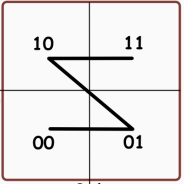
\includegraphics[width=30mm,keepaspectratio]{images/zcell.png}
% \caption{Morton curve traversing pattern \label{zcell}}
% \endminipage \hfill
% \minipage{0.4\linewidth}
% \centering
% 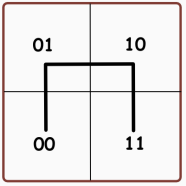
\includegraphics[width=30mm,keepaspectratio]{images/hilbertcell.png}
% \caption{Hilbert curve traversing pattern \label{hilbertcell}}
% \endminipage \hfill
% \end{figure}

\subsection{Flexibile load balancing}

As mentioned earlier most of the partitioning schemes are focused on uniform distribution of tasks across all the processor. The main drawback of this approach is, the uniform-work load balancing can cause
imbalance in the communication load, slowing down the overall computation. In this paper we introduce some flexibility to the load balancing in order to reduce the overall communication
costs. 
% and reduce the overall execution time of the computation. 
To demonstrate the above claim we conduct two experiments, a) Standard SFC based partition, where the work is uniform across all processes and compare the communication (using the surface area of the partition as a surrogate), and b) A flexible SFC based partition, where we allow a small 'slack' (say at most $10\%$ of $N/p$) of the work that each process gets. 
% \begin{itemize}
% \item Standard SFC based partition, where the work is uniform across all processes and compare the communication (using the surface area of the partition as a surrogate)
% \item A flexible SFC based partition, where we allow a small 'slack' (say at most $10\%$ of $N/p$) of the work that each process gets. 
% \end{itemize}

%\begin{multicols}{2}
\begin{figure}[t]
\centering
\includegraphics[height=3.5cm,keepaspectratio]{images/nca1.pdf}
%\caption{Refined Hilbert curve covering the points $p_1\ and \ p_2$ \label{zcell}}
%\end{figure}
%\begin{figure}[H]
%\centering
\includegraphics[height=3.5cm,keepaspectratio]{images/nca2.pdf}
\caption{Ordering of points based on the Rotation pattern inside the NCA \label{hilbertcell}}
\end{figure}
%\end{multicols}

\section{Results}
Baseline and NCA based Hilbert and Morton ordering algorithms are executed with varying maximum depth for sorting one million (2D \& 3D) points. 
% In this context maximum depth refers to the maximum height of the octree needed to compute the Hilbert or Morton ordering. 
Each implementation of the Hilbert and Morton ordering executed twenty times and mean executing time in milliseconds is taken as the performance measure.
Fig.\ref{3d_NCA} depict the 2D and 3D Hilbert and Morton ordering performance for different implementations. All the SFC implementations are run in Intel Xeon E7-4820v2 CPU @2.00 GHz (32 cores) processor
with 64 GB DDR3 RAM and using the g++ 4.8 compiler in the Ubuntu 14.04 LTS environment. 
% \begin{itemize}
%  \item {\bf convert this to a single sentence instead of itemized}
%  \item Intel Xeon E7-4820v2 CPU @2.00 GHz (32 cores)
%  \item RAM: 64 GB DDR3
%  \item OS: Ubuntu 14.04 LTS
%  \item Compiler: g++ 4.8
% \end{itemize}

% {\bf 1-2 sentences summarizing the results of fig 2d and 3d. Also 1 sentence concluding.} 
According to the Fig.\ref{3d_NCA}, we can see that the execution time of recursive approach resides in the range of 10s to 40s, while the execution time of the NCA approach
is less than 3s (in 2D implementation) and 4.5s (in 3D implementation). 
% If we consider the Morton baseline and Morton NCA implementations, we can see that Morton NCA implementation is outperformed by the Morton baseline implementation when the maximum depth parameter exceeds 7 (in 2D implementation) and 4 (in 3D implementation). 
In the average case, Morton NCA and Morton baseline performances are very close to each other. Our results suggest that the NCA based Hilbert ordering is 9 times faster (mean performance) than the traditional recursive Hilbert
ordering and the NCA property can be used to calculate the ordering of a generic SFC efficiently. 

%\vspace{-0.3in}
% \begin{figure}[tbh]
% \centering
% \begin{tikzpicture}
% \pgfplotsset{width=4.5cm,compat=1.9}
% \begin{axis}[
% 	x tick label style={
% 		/pgf/number format/1000 sep=},
% 	ylabel=Execution Time (ms),
% 	enlargelimits=0.05,
% 	legend style={at={(0.4,-0.2)},
% 	anchor=north,legend columns=-1},
% 	ybar interval=0.7,
% ]
% 
% \addplot %Hilbert Baseline 2D
% coordinates{
% (2,2113.2)
% (4,5568.55)
% (6,11155.1)
% (8,19654.2)
% (10,26824.8)
% (12,0)
% };
% 
% \addplot % Hilbert NCA
% coordinates {
% (2,910.7)
% (4,1197.8)
% (6,1683.6)
% (8,2402.8)
% (10,3370.5)
% (12,0)
% };
% 
% \addplot %Morton Baseline
% coordinates{
% (2,1058.45)
% (4,1060.8)
% (6,1135)
% (8,1284.6)
% (10,1543.65)
% (12,0)
% };
% 
% \addplot %Morton NCA
% coordinates{
% 
% (2,836.55)
% (4,955.7)
% (6,1141.75)
% (8,1410.8)
% (10,1864.9)
% (12,0)
% };
% 
% \legend{Hilbert BL,Hilbert NCA, Morton BL, Morton NCA}
% \end{axis}
% 
% 
% 
% \end{tikzpicture}
% \caption{2d ordering of points for Hilbert and Morton baseline, Hilbert and Morton NCA approaches.\label{2d_NCA}}
% \end{figure}

\begin{figure}[tbh]
\centering
\begin{tikzpicture}
\pgfplotsset{width=7.5cm,compat=1.9}
\begin{axis}[
	x tick label style={
		/pgf/number format/1000 sep=},
        ylabel=Execution Time (ms),
	enlargelimits=0.05,
	legend style={at={(0.4,-0.2)},
	anchor=north,legend columns=-1},
	ybar interval=0.7,
	xbar bar width=0.1cm
	enlarge x limits=0.07	
]


\addplot % Hilbert Baseline 3D
coordinates {
(2,5494.05)
(4,17982)
(6,39330.2)
(8,46483.6)
(10,46684.9)
% (15,46578.8)
% (30,46803.8)
(12,10)
};


\addplot % Hilbert NCA
coordinates {
(2,2606.2)
(4,3655.95)
(6,4632.3)
(8,5103.65)
(10,5333.15)
% (15,5880.2)
% (30,7758.5)
(12,10)
};

\addplot %Morton Baseline
coordinates{
(2,2140.85)
(4,2562.7)
(6,2779.6)
(8,2990.65)
(10,2915.3)
% (15,2882.4)
% (30,2919.95)
(12,10)
};

\addplot %Morton NCA
coordinates{
(2,2001.9)
(4,2611.75)
(6,3052.65)
(8,3610.1)
(10,3771.6)
% (15,4324.25)
% (30,6488.5)
(12,10)

};



\legend{Hilbert BL,Hilbert NCA, Morton BL, Morton NCA}
\end{axis}
\end{tikzpicture}
\caption{3d ordering of points for Hilbert and Morton baseline, Hilbert and Morton NCA approaches.\label{3d_NCA}}
\end{figure}

In the second experiment we allow some flexibility to the load, and observe how contour ratio (ratio between the surface area of the mesh that each node gets with flexibility, Vs 0 flexibility case)
behaves with Hilbert and Morton ordering based partitioning. Our results show that (see Fig.\ref{flexibility}) by using the Hilbert ordering we can achieve low contour ratios compared with the Morton ordering which implies low
communication costs.
% We can conclude that by using Hilbert ordering with some flexibility we can reduce communication costs further compared to the Morton ordering (even with some flexibility).

\begin{figure}[tbh]
\centering
\includegraphics[height=5cm,keepaspectratio]{images/flexPart.pdf}
\caption{ Flexible partitioning results using Hilbert and Morton ordering \label{flexibility}}
\end{figure}
\section*{Conclusions}
In this work we presented a faster algorithm for computing the ordering of SFCs, specifically the Hilbert curve. We also demonstrated the improvement in partitioning quality by allowing for non-uniform assignment of work. Future work will focus on testing this for larger clusters and actual communication costs. 
%\begin{itemize}
%\item Hilbert ordering is better than Morton ordering in terms of preserving the geometric locality of objects. 
%\item We can conclude that the NCA based Hilbert ordering algorithm is 9 times faster than the traditional recursive approach for Hilbert ordering. 
% \item NCA based algorithm is easily extensible to compute the ordering of any generic SFC (i.e. Morton, Peano etc.)
%\item Allowing some flexibility to the load at each node can reduce the communication further  (approximately in the range of 1.125-1.175 times), and reduce the overall computation time. 
%\end{itemize}
\bibliographystyle{abbrv}
\bibliography{hilbert} 

\end{document}
